\documentclass[paper.tex]{subfiles}

\usepackage{tikz}
\usepackage{amsmath}
\usepackage{graphicx}
\usepackage{tabularx}
\usepackage{multicol}
\usepackage{algpseudocode}
\usepackage{algorithm}

% Add vertical spacing to tables
\renewcommand{\arraystretch}{1.4}

% Begin Document
\begin{document}

\begin{center}
    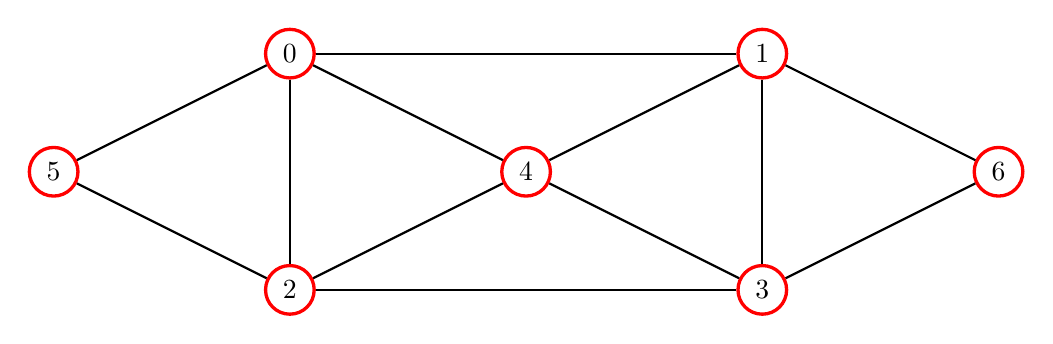
\begin{tikzpicture}
    
        \begin{scope}[every node/.style={circle,very thick,draw=red}]
            \node (1) at (0,3) {0};
            \node (2) at (6,3) {1};
            \node (3) at (0,0) {2};
            \node (4) at (6,0) {3};
            \node (5) at (3,1.5) {4};
            \node (6) at (-3,1.5) {5};
            \node (7) at (9, 1.5) {6};
        \end{scope}

        \begin{scope}[every edge/.style={draw=black,thick}]
            \path [-] (6) edge node {} (1);
            \path [-] (6) edge node {} (3);
            \path [-] (1) edge node {} (3);
            \path [-] (1) edge node {} (2);
            \path [-] (1) edge node {} (5);
            \path [-] (3) edge node {} (5);
            \path [-] (3) edge node {} (4);
            \path [-] (2) edge node {} (5);
            \path [-] (5) edge node {} (4);
            \path [-] (4) edge node {} (2);
            \path [-] (2) edge node {} (7);
            \path [-] (4) edge node {} (7);
        \end{scope}
    
    \end{tikzpicture}
\end{center}

\end{document}